%\documentclass[tikz, border=5pt]{standalone}
\usetikzlibrary{angles, quotes, shapes.geometric} % 加载角度、引用、直角标记库
\begin{document}
	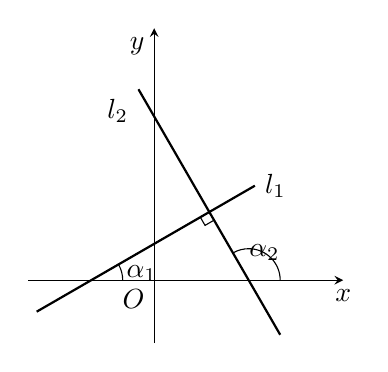
\begin{tikzpicture}[>=stealth, scale=0.8]

    % 1. 绘制坐标轴
    \draw[->] (-2,0) -- (3,0) node[below] {$x$}; % x轴(带箭头和标签)
    \draw[->] (0,-1) -- (0,4) node[below left] {$y$}; % y轴(带箭头和标签)
    \node at (0,0) [below left] {$O$}; % 原点标记

    % 2. 绘制直线 \( l_1 \)(倾斜向上)
    \draw[thick] (-1, 0) --  ++(30: 3) node[right] {$l_1$};
    \draw[thick] (-1, 0) --  ++(-150: 1) ;
    
    % 3. 绘制直线 \( l_2 \)(倾斜向下,与 \( l_1 \) 垂直)
    \draw[thick] (1.5, 0) -- ++(120: 3.5) node[below left] {$l_2$};
    \draw[thick] (1.5, 0) -- ++(-60: 1) ;
    
    % 4. 标记角度 \( \alpha_1 \)(\( l_1 \) 与 x 轴正方向的锐角)
    \draw (-0.5, 0) arc (0:30:0.5) ;
    \node at (-0.2, 0.1) []  {$\alpha_1$}; 

    % 5. 标记角度 \( \alpha_2 \)(\( l_2 \) 与 x 轴正方向的钝角)
    \draw (2, 0) arc (0:120:0.5) node[midway] {$\alpha_2$}; 
    
    % 6. 绘制直角标记(两直线垂直的符号)
    \draw (-1, 0) --  ++(30: 2) -- ++(-60: 0.15) -- ++(30: 0.15) ;

	\end{tikzpicture}
\end{document}
